% DSA4213 Assignment 1 report, first draft of the setup sections (12 Oct 2026).
% Compile: pdflatex main && bibtex main && pdflatex main && pdflatex main
% Tables in tables/ and figures in figures/ are written by
% scripts/make_report_figures.py from the result files; do not edit them by hand.
% Red text marks drafting notes. Remove every \todo before submitting.

\documentclass[11pt]{article}
\usepackage[preprint]{acl}

\usepackage{times}
\usepackage{latexsym}
\usepackage[T1]{fontenc}
\usepackage[utf8]{inputenc}
\usepackage{microtype}
\IfFileExists{inconsolata.sty}{\usepackage{inconsolata}}{} % Overleaf has it
\usepackage{graphicx}
\usepackage{booktabs}
\usepackage{amsmath}
\usepackage{tabularx}
\usepackage{enumitem}
\usepackage{placeins}

\newcommand{\tok}[1]{\texttt{<#1>}}
\newcommand{\todo}[1]{\textcolor{red}{[#1]}}
\newcommand{\Jtest}{J_{\text{test}}}
\graphicspath{{figures/}}
\setlength\titlebox{4.6cm} % default 5.2cm; our title and author block fit in less

\title{Does Better Next-Token Prediction Give Better Text Representations,\\
and What Does Each Model Family Pay for It?}

\author{Lee Kai Rong, Student ID: A0287723U \\
  National University of Singapore \\
  Code: \todo{GitHub link}}

\begin{document}
\maketitle

\begin{abstract}
We compare four kinds of next-token language model, an interpolated 5-gram, an RNN, an LSTM and a Transformer, on English reviews of beauty products; the three neural models have core sizes within 2.3\% of each other and share one training recipe. We then change only one model's input embeddings (learned with the model, our own vectors kept fixed, or public GloVe vectors kept fixed), and finally freeze the models to test whether those that predict text best also give the best features for sentiment classification. \todo{Two or three sentences with the headline results of Parts I to III, written after the runs.}
\end{abstract}

%=====================================================================
\section{Question and Setup}
\label{sec:setup}

We ask one question across the three parts: \emph{does better next-token prediction give better text representations, and what does each model family pay for it?} Each comparison holds the data and tokens fixed, and the neural models share one training recipe.

\paragraph{Corpus.}
We use the All\_Beauty reviews of Amazon Reviews 2023 \citep{hou2024bridging}: 701,528 reviews of 112,565 products with 1 to 5 stars. The stars give in-domain labels for Part~III; we split by product ourselves, so no test product reaches language-model training; and reviews are very unlikely to be in Wikipedia or Gigaword, the text behind Part~II's GloVe vectors \citep{carlson2025new} (Table~\ref{tab:corpora}).

\paragraph{Preprocessing.}
Cleaning turns HTML tags, links and e-mail addresses into spaces, decodes HTML entities and maps numbers to \tok{num}; the course tokenizer \citep{zhou2026notebooks} keeps lowercase a--z words, contractions whole, and six punctuation marks. Four filters, applied before the split and set from measurements on this data (Appendix~\ref{app:data}), remove 114,395 reviews, leaving 587,133 (21.2M tokens) of 111,348 products (Table~\ref{tab:data}):
(i)~reviews with no word or over 512 tokens, so one Transformer context holds every review; short reviews stay, since a 3-word minimum would drop 8.7\% of positive but 3.4\% of negative reviews;
(ii)~non-English reviews, judged by fastText \citep{joulin2017bag} and, below seven words, where fastText is unreliable, by a word score learnt from our reviews;
(iii)~repeats by the same person and exact copies of 14+ words by different people \citep{lee2022deduplicating}, since different people write near-identical reviews of up to 13 words but none of 14 to 26;
(iv)~reviews beyond 90 per product, chosen at random: a few products dominate (the top 1\% hold 28\% of reviews), and with a within-product rating correlation of $\rho = 0.17$, 90 reviews estimate a product's mean rating with 95\% of the precision any number could \citep{kish1965survey}.

\begin{table}[t]
\centering
\small
\setlength{\tabcolsep}{3.5pt}
\begin{tabular}{@{}lrr@{}}
\toprule
Corpus step & Reviews & Share \\
\midrule
Raw All\_Beauty reviews & 701,528 & \\
\quad $-$ no word, or over 512 tokens & 2,583 & 0.4\% \\
\quad $-$ not English & 11,634 & 1.7\% \\
\quad $-$ duplicates & 8,209 & 1.2\% \\
\quad $-$ over 90 per product & 91,969 & 13.5\% \\
Clean corpus & 587,133 & 83.7\% \\
\midrule
Pile (split keys) & Reviews & Size \\
\midrule
LM training $[0, 0.5)$ & 295,645 & 10.96M targets \\
LM validation $[0.5, 0.55)$ & 28,505 & 1.07M targets \\
LM test $[0.55, 0.6)$ & 29,827 & 1.12M targets \\
Part III test $[0.6, 0.7)$ & 57,288 & 24,362 bal. \\
Part III training $[0.7, 1)$ & 175,868 & 74,344 bal. \\
\bottomrule
\end{tabular}

\caption{From raw reviews to piles. Shares are of the reviews entering each step; targets are tokens plus \tok{eos}; Part~III sets balance 1--2 star (negative) and 4--5 star (positive) reviews.}
\label{tab:data}
\end{table}

\paragraph{Splits and vocabulary.}
Each product gets one random split key (seed 4213), and each pile is a range of keys (Table~\ref{tab:data}), so piles share no product, though short everyday reviews recur across people (Table~\ref{tab:limits}). Training covers every product the test run of Appendix~\ref{app:training} saw. Validation and test take 5\% each, on which a unigram model's $J$ has a standard error of about 0.003 nats. The vocabulary keeps tokens seen at least five times in training, plus \tok{pad}, \tok{unk}, \tok{bos} and \tok{eos} ($|V| = 17{,}068$); \tok{unk} is 0.60\% of test targets.

\paragraph{Scoring.}
All models face the same prediction problem \citep[slide~29]{zhou2026lecture3}: the same text, vocabulary and targets, and no context from outside the review. Each review is scored on its own from $x_1 = \tok{bos}$; review $r$ has $T_r$ targets (its tokens and \tok{eos}), $N = \sum_r T_r$, and
\begin{equation}
\Jtest = \frac{1}{N}\sum_{r}\sum_{t=1}^{T_r} -\log P_\theta\big(x^{(r)}_{t+1} \,\big|\, x^{(r)}_{1:t}\big),
\label{eq:j}
\end{equation}
with $\mathrm{PPL} = \exp(\Jtest)$. Padding is masked, and the code asserts the same $N$ for every model (1,115,210 test targets). The Transformer's context, $L = 513$, holds the longest review plus \tok{bos}, so no neural model needs a sliding window.

%=====================================================================
\section{Part I: Four Language Models}
\label{sec:part1}

\subsection{Models and training}
\label{sec:models}

\begin{table}[t]
\centering
\small
\setlength{\tabcolsep}{4pt}
\begin{tabular}{@{}llll@{}}
\toprule
Model & Size & Context & Tuned \\
\midrule
Kneser-Ney 5-gram & 19.7M $n$-grams & last 4 & $n$ \\
Add-$k$ 5-gram & 19.7M $n$-grams & last 4 & $n$, $k$, $\lambda$ \\
RNN, $H{=}512$ & 365,668 & all so far & peak LR \\
LSTM, $H{=}248$ & 372,100 & all so far & peak LR \\
Transformer & 374,200 & all so far & peak LR \\
\bottomrule
\end{tabular}

\caption{Part~I models. Neural sizes are core parameters; each also has the same 3,430,668 word-table parameters. Tuned settings use validation $J$.}
\label{tab:models}
\end{table}

\paragraph{$n$-gram models.}
We wrote our own interpolated modified Kneser-Ney \citep{chen1998empirical}, the $n$-gram baseline in Lecture~3's benchmark table \citep{chelba2013one}, and the course's interpolated add-$k$ \citep{zhou2026notebooks}, so both share the neural models' vocabulary, targets and target-count check. The order $n \le 5$, and add-$k$'s $k$ and weights $\lambda$ \citep[by EM;][]{jurafsky2026speech}, are chosen on validation data; both choose $n = 5$, which beats $n = 4$ by only 0.003 nats for Kneser-Ney.

\paragraph{Neural models.}
The RNN \citep[Elman, $\tanh$;][]{elman1990finding} and the LSTM \citep{hochreiter1997long} have one layer of $H = 512$ and 248 units. The Transformer has three causal decoder layers ($d_{\text{model}} = 100$, 4 heads, $d_{\text{ff}} = 400$) with layer normalisation before each sub-layer \citep[pre-LN;][]{xiong2020layer} and sinusoidal positions \citep{vaswani2017attention}. All three share the input table $E$ ($|V| \times 100$, a GloVe size, so Part~II can reuse a Part~I model) and the output layer, untied because Part~II freezes $E$. Their cores, everything else, match within 2.3\% in parameters (Table~\ref{tab:models}), so architectures are compared at equal size without the vocabulary tables \citep{kaplan2020scaling,collins2017capacity}. Versions of these main models (S) with about four times the core (M) check the effect of size. \todo{Confirm after the M runs.}

\paragraph{Training.}
Only the peak learning rate is tuned per model, by one rule for all \citep{dodge2019show}: $3\times10^{-4}$, $10^{-3}$ and $3\times10^{-3}$, then half-decade steps further while the best rate is the largest or smallest tried \citep{bengio2012practical}. Every try is a complete planned run, and the best try becomes the final model. Shared and fixed in advance (Table~\ref{tab:recipe}): AdamW; 8,192 positions per batch, padding included (about 7,000 targets); warm-up, then cosine decay over a budget of 6 epochs; gradient clipping; and early stopping on validation $J$, checked four times per epoch. Dropout is 0, and a fixed training sample scored at every check tests for overfitting under a rule set in advance (Appendix~\ref{app:rules}). Neural models train on an Apple M4 laptop GPU (PyTorch MPS, 16~GiB), $n$-gram models on its CPU.

\subsection{Prediction quality}
\todo{Table 3: validation and test $J$ and PPL for all models (plus add-$k$), \tok{unk} share, chosen learning rates and the tries per model. Paragraph: observation with numbers, then hedged explanations.}

\subsection{Cost}
\todo{Training time, time to best checkpoint, parameters, stored $n$-grams, memory, inference throughput on one common workload, timing procedure (D1.7).}

\subsection{Learning behaviour}
\todo{Figure 1: training, training-sample and validation $J$ against targets seen, one colour per model (D1.8). Convergence and overfitting against the rules of Appendix~\ref{app:rules}.}

\subsection{Generated text}
\todo{Fixed prompts, matched decoding (D1.6), samples chosen by a rule set in advance; repetition, local fluency, consistency.}

%=====================================================================
\section{Part II: Embedding Variants}
\label{sec:part2}
\todo{About 1.1 pages: held-constant table, coverage, test $J$, convergence, stability over seeds, cost of our own embeddings.}

\section{Part III: Downstream Representations}
\label{sec:part3}
\todo{About 1.1 pages: representations, classifier protocol, accuracy with intervals, errors by length group, language-model versus downstream ranking.}

\section{Synthesis, Limitations and Lessons}
\label{sec:synthesis}
\todo{About 0.5 page: the answer to the question across the three parts, the main limitations, lessons learned. Code, data licence and AI use: Appendix~\ref{app:repro}.}

%=====================================================================
\bibliography{references}

\appendix
\counterwithin{figure}{section}
\counterwithin{table}{section}
\renewcommand{\thefigure}{\thesection\arabic{figure}}
\renewcommand{\thetable}{\thesection\arabic{table}}

%=====================================================================
\section{Data and Preprocessing Evidence}
\label{app:data}

\paragraph{Choice of corpus.}
Table~\ref{tab:corpora} compares the seven corpora we considered. WikiText-2 is a standard language-modelling benchmark, but it is Wikipedia text, which GloVe was trained on, so Part~II's public vectors would have seen it. IMDB has sentiment labels and little overlap with GloVe, but its 50,000 unlabelled reviews, the natural language-model training text, are not documented as disjoint by movie from its labelled test set \citep{maas2011learning}. Amazon Movies \& TV has the same properties as All\_Beauty with about 25 times as many reviews; as the assignment allows, we took the category whose size suits one laptop.

\begin{table}[t]
\centering
\small
\setlength{\tabcolsep}{3pt}
\begin{tabular}{@{}lccc@{}}
\toprule
Corpus & Labels & Item split & Not in GloVe \\
\midrule
WikiText-2 & none & -- & no \\
AG News & topics & no & partly \\
TinyStories & none & -- & yes \\
Gutenberg novels & to build & yes & yes \\
IMDB & sentiment & partly & yes \\
Amazon Movies \& TV & stars & yes & yes \\
Amazon All\_Beauty & stars & yes & yes \\
\bottomrule
\end{tabular}
\caption{Candidate corpora. Labels: in-domain labels for Part~III (Gutenberg's, such as authorship, would have to be built). Item split: all text about one product, movie or book can be kept on one side of every split, so no Part~III test item appears in language-model training (-- where there are no labels). Not in GloVe: the text is unlikely to be in GloVe's Wikipedia and Gigaword training data (AG News is news, like Gigaword).}
\label{tab:corpora}
\end{table}

\begin{figure*}[t]
\centering
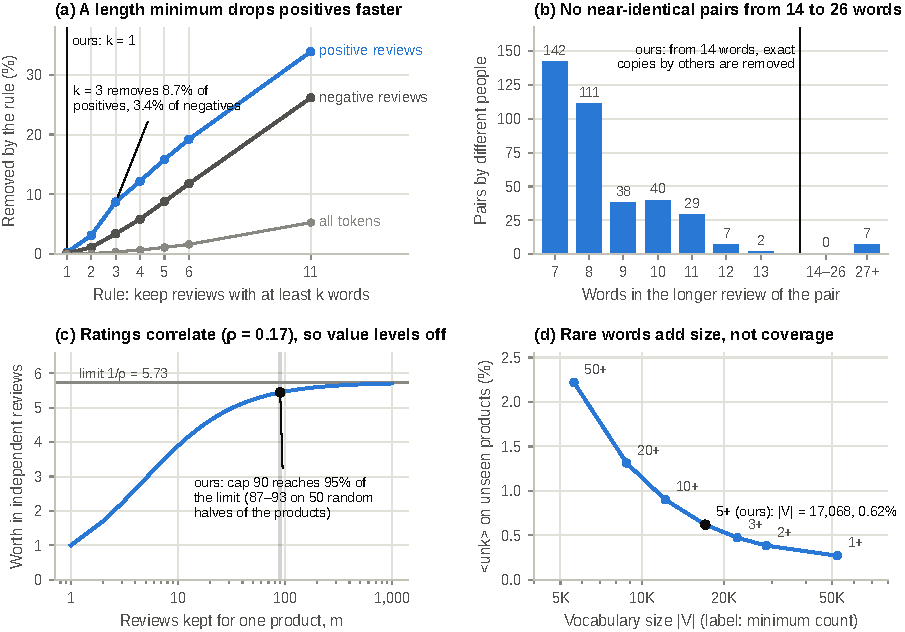
\includegraphics[width=\textwidth]{preprocessing.pdf}
\caption{The measurement behind four preprocessing thresholds; black marks our choice.
(a)~Share of positive (4--5 stars) and negative (1--2 stars) reviews, and of all tokens, that a minimum of $k$ words would remove (raw reviews after cleaning). We only remove reviews with no word ($k = 1$).
(b)~Pairs of near-identical but not identical reviews by different people, sharing 90\% or more of their distinct words, by the length of the longer review (final corpus, exact search; \citealp{chaudhuri2006primitive,bayardo2007scaling}). Below 14 words such pairs are everyday sentences, and exact copies of them are kept; from 14 words, exact copies by different people are removed. The 7 pairs of 27 or more words read as copies and remain (Table~\ref{tab:limits}).
(c)~Kish's design effect with the intraclass correlation of star ratings within a product, $\rho = 0.1745$: $m$ reviews are worth $m/(1+(m-1)\rho)$ independent ones, approaching $1/\rho = 5.73$. A cap of 90 reaches 95\%; the grey band is the cap's range (87 to 93) when $\rho$ is re-estimated on 50 random halves of the products.
(d)~Vocabulary built on the products with keys below 0.5 (the later training pile) and tested on the rest; labels give the minimum count.}
\label{fig:preprocessing}
\end{figure*}

\paragraph{Cleaning.}
Before tokenizing, Amazon video tags (in 5,951 reviews) become spaces, links to other products keep the product name (474 reviews), e-mail addresses are removed as personal data (42 reviews), ``\&'' becomes ``and'' and curly apostrophes are straightened. The course tokenizer is the regular expression \texttt{[a-z]+(?:'[a-z]+)?|[.,!?;:]} on lowercased text, extended to keep \tok{num} whole.

\paragraph{Lengths.}
Reviews under three words are 7.2\% of reviews but hold 0.4\% of tokens, and a minimum length would change the label mix (Figure~\ref{fig:preprocessing}a), so we keep them. The 512-token limit removes 723 reviews (0.10\%) and lets one Transformer context of 513 positions hold every review with its \tok{bos}.

\paragraph{English only.}
fastText's language identifier \citep{joulin2017bag,joulin2016fasttextzip}, its compressed lid.176 model used through the fast-langdetect package, would on its own remove 15,434 reviews, a third of them of one or two words, where its guesses are least reliable: of 25 one- or two-word reviews it labelled non-English with probability below 0.5, only 11 were foreign. Curly apostrophes also made it label English reviews as Russian or Thai, so they are straightened first. Our word score sums, over a review's words, the log of how much more often each word appears in non-English than in English reviews (a score of 2 means about 7 times). It is learnt from reviews of seven or more words that fastText labels with probability 0.9 or more (516,880 English, 5,090 other), so it inherits fastText's labels. Reviews of up to six words are removed when their score is 2 or more. Longer reviews are removed when fastText's top language is not English and either it is at least 90\% sure or the score is 2 or more, and also when a sentence of five or more words is non-English for fastText (probability 0.9 or more) with an average word score of 2 or more, as in an English review followed by a translation. The rule keeps 3,997 reviews that fastText flagged, almost all of them short (Table~\ref{tab:language}). Filtering a language-model corpus by language and duplicates follows C4 \citep{raffel2020exploring}.

\begin{table}[t]
\centering
\small
\setlength{\tabcolsep}{4pt}
\begin{tabular}{@{}lrrrr@{}}
\toprule
Words & Reviews & fastText & Our rule & Flags kept \\
\midrule
1–2 & 48,903 & 4,953 & 2,608 & 2,546 \\
3–6 & 89,885 & 4,192 & 2,945 & 1,271 \\
7–20 & 226,260 & 4,446 & 4,270 & 177 \\
21+ & 333,894 & 1,843 & 1,849 & 3 \\
\midrule
All & 698,942 & 15,434 & 11,672 & 3,997 \\
\bottomrule
\end{tabular}

\caption{Reviews removed as not English, by length in words: by fastText's top guess alone and by our rule; flags kept are fastText flags that our rule keeps. From the run that designed the rule (698,942 reviews); the final pipeline removed 11,634 (Table~\ref{tab:data}). \todo{Regenerate from the final rule: rerun scripts/explore\_language.py.}}
\label{tab:language}
\end{table}

\paragraph{Duplicates.}
Exact copies by the same person are one review counted again (8,021 removed), and near copies by the same person share 90\% or more of their distinct words (69 removed). A first line of 7 words for exact copies by different people removed mostly everyday sentences (8 of 10 in a hand-checked sample), so it moved to 14: on the final corpus, near-identical but not identical reviews by different people occur at every length from 7 to 13 words and never from 14 to 26 (Figure~\ref{fig:preprocessing}b). Exact copies of 14 or more words by different people are removed (119).

\paragraph{Cap per product.}
Before the cap, the top 1\% of products held 28\% of reviews and one product had 1,962. Star ratings of one product correlate, with intraclass correlation $\rho = 0.1745$. By Kish's design effect, $m$ reviews of a product estimate its mean rating as precisely as $m/(1+(m-1)\rho)$ independent reviews would, which approaches $1/\rho = 5.73$; 90 is the smallest $m$ that reaches 95\% of that limit. Re-estimated on 50 random halves of the products, $\rho$ ranges from 0.170 to 0.181 and the cap from 87 to 93 (Figure~\ref{fig:preprocessing}c). Kept reviews are chosen by a fixed random number per review (seed 4213).

\paragraph{Pile sizes.}
Pile sizes come from 20 slices of 5\% of the split keys. On every slice a unigram model's $J$ has a standard error of 0.0030 to 0.0035 nats when reviews are resampled, so 5\% is enough for validation and for test; this ignores the correlation between reviews of one product and the variation between training seeds. Training must cover $[0, 0.5)$ because the test run used products from that range. Larger training piles would lower every model's $J$ somewhat but shrink Part~III's balanced training set from 74,344 reviews to about 49,700 (training on $[0, 0.6)$, Part~III training on $[0.7, 0.9)$) or 24,700 (training on $[0, 0.7)$, Part~III training on $[0.9, 1)$); how the ranking changes with more training data is not tested.

\paragraph{Vocabulary.}
The cut-off was measured by building a vocabulary on the products with keys below 0.5, which later became the training pile, and counting \tok{unk} on the other half; swapping the halves gives the same curve (Figure~\ref{fig:preprocessing}d). Lowering the minimum count from 10 to 5 adds 4,918 words and removes 0.28 percentage points of \tok{unk}; lowering it further to 3, 2 and 1 adds 5,279, 6,278 and 23,618 words for 0.15, 0.09 and 0.11 points. Five is also gensim word2vec's default minimum count \citep{rehurek2010software}, so Part~II's own embeddings see every vocabulary word at least five times.



\paragraph{Hand checks.}
We read random samples of each rule's decisions (seed 4213) and counted those the rule got right (Table~\ref{tab:handchecks}). Claude, the AI assistant used in this project (Appendix~\ref{app:repro}), counted the same samples. The counts agree on 7 of 8 samples. For samples 1 to 6 the author had seen Claude's counts before counting; for 7 and 8 the author counted first. The one disagreement is a review whose only non-English words are a five-word holiday greeting: the author counted it as containing a foreign sentence, Claude did not. Samples of 10 are small: 10 of 10 right still allows an error rate of up to 26\% (one-sided 95\% bound).

\begin{table}[t]
\centering
\small
\setlength{\tabcolsep}{3pt}
\begin{tabular}{@{}rlrrr@{}}
\toprule
\# & Sample & $n$ & Author & Claude \\
\midrule
1 & Removed, 1--6 words & 40 & 40 & 40 \\
2 & Removed, 7+ words & 40 & 40 & 40 \\
3 & Removed, foreign sentence & 28 & 28 & 27 \\
4 & Kept, 1--6 words, flagged & 30 & 30 & 30 \\
5 & Kept, 7+ words, flagged & 30 & 29 & 29 \\
6 & Removed, own near copy & 10 & 10 & 10 \\
7 & Removed, 14+ word copy by other & 10 & 10 & 10 \\
8 & Kept, 7--13 word copy by other & 10 & 10 & 10 \\
\bottomrule
\end{tabular}
\caption{Hand checks: reviews the rule got right in a random sample of $n$ (sample 3 holds all 28 such removals). Flagged: fastText's top guess was not English. Own near copy: by the same person; by other: by a different person. Right means not English (1, 2); contains a non-English sentence (3); English (4, 5); the same review again (6); copied, not written independently (7); an everyday sentence anyone could write (8).}
\label{tab:handchecks}
\end{table}

\begin{table}[t]
\centering
\small
\setlength{\tabcolsep}{3pt}
\begin{tabular}{@{}lr@{}}
\toprule
Check & Result \\
\midrule
Rows, tokens, fingerprint match the report & yes \\
A rerun gives a byte-identical file & yes \\
Tokens outside the tokenizer's pattern & 0 \\
Review length & 1 to 512 tokens \\
Reviews per product & at most 90 \\
Products with more than one split key & 0 \\
Products per tenth of the keys & 11,000 to 11,237 \\
Same-person repeats & 0 \\
14+ word copies by different people & 0 \\
E-mail addresses left & 0 \\
Reviews with 4+ foreign function words & 2 \\
\bottomrule
\end{tabular}
\caption{Checks on the clean corpus; every rule holds. The last row counts leftovers that remain as a limitation.}
\label{tab:checks}
\end{table}

\begin{table}[t]
\centering
\small
\setlength{\tabcolsep}{4pt}
\begin{tabularx}{\columnwidth}{@{}lr>{\raggedright\arraybackslash}X@{}}
\toprule
Limitation & Share & Consequence \\
\midrule
Numbers become \tok{num} & 15.9\% & ``0 stars'' and ``5 stars'' look alike \\
Reviews by repeat users & 14.5\% & a user's style may reach several piles \\
Short repeats kept & 7.4\% & a short review can be in training and test \\
Runs of punctuation & 2.2\% & 0.34\% of tokens, the same for every model \\
Emoji dropped & 2.0\% & some sentiment signal lost \\
Reviews over 512 tokens & 0.10\% & 2.0\% of tokens removed \\
Contractions split & 0.06\% & odd apostrophes give ``don~t'' \\
Accented words split & $\ge$0.05\% & ``cr\`eme'' becomes ``cr~me'' \\
Long near copies & 7 pairs & 2 of them span two products \\
\bottomrule
\end{tabularx}
\caption{Measured limitations of the preprocessing. Shares are of reviews in the clean corpus, except numbers, emoji and long reviews (raw reviews).}
\label{tab:limits}
\end{table}

\paragraph{Checks on the final corpus.}
A script reruns these checks on the file the models read (Table~\ref{tab:checks}). The corpus fingerprint (SHA-256 of the uncompressed file) starts \texttt{16ec4ec1}, so anyone who rebuilds the corpus can confirm it is identical.



\paragraph{Limitations.}
Each limitation of the preprocessing is measured (Table~\ref{tab:limits}). Every filter was designed on the whole corpus before the split, and none used a model result, but some used text or ratings of products that later became evaluation products: the length rule compared the label mix of all reviews, the word score was learnt from all reviews, the cap's $\rho$ uses every product's ratings, and the vocabulary cut-off was compared on the other half of the products. These choices barely depend on which products became test products: the cap moves only between 87 and 93 across random halves of the products, and swapping the vocabulary halves gives the same curve.



%=====================================================================
\section{Model and Training Evidence}
\label{app:training}

\begin{table*}[t]
\centering
\small
\begin{tabular}{@{}lrrrrrrrr@{}}
\toprule
 & & \multicolumn{2}{c}{K targets/s} & Memory & Noise & Mean & Clipped & $J$ after \\
\cmidrule(lr){3-4}
Model & Core & 8K & 16K & 8K (GiB) & scale & norm & steps & 300 steps \\
\midrule
RNN-S & 365,668 & 44.0 & 43.2 & 3.9 & 13,095 & 0.96 & 23\% & 5.726 \\
LSTM-S & 372,100 & 44.2 & 43.4 & 3.9 & 8,060 & 0.71 & 11\% & 5.812 \\
Transformer-S & 374,200 & 40.6 & 40.2 & 4.0 & 23,909 & 0.67 & 11\% & 5.028 \\
RNN-M & 1,480,740 & 34.8 & 37.9 & 3.8 & 15,407 & 1.21 & 41\% & 5.718 \\
LSTM-M & 1,489,500 & 37.6 & 37.1 & 4.1 & 10,480 & 0.87 & 17\% & 5.699 \\
Transformer-M & 1,578,980 & 32.5 & 32.0 & 4.8 & 11,722 & 0.76 & 11\% & 4.963 \\
\bottomrule
\end{tabular}

\caption{Test run: core parameters, training speed at 8K and 16K positions per batch, peak memory at 8K, gradient noise scale $B_{\text{simple}}$ at step 300 (targets), mean unclipped gradient norm and share of clipped steps over the second half of the run, and validation $J$ after 300 steps. S models are the main size; M models are the size check, with cores matched within 6.6\%.}
\label{tab:pilot}
\end{table*}

\begin{figure*}[t]
\centering
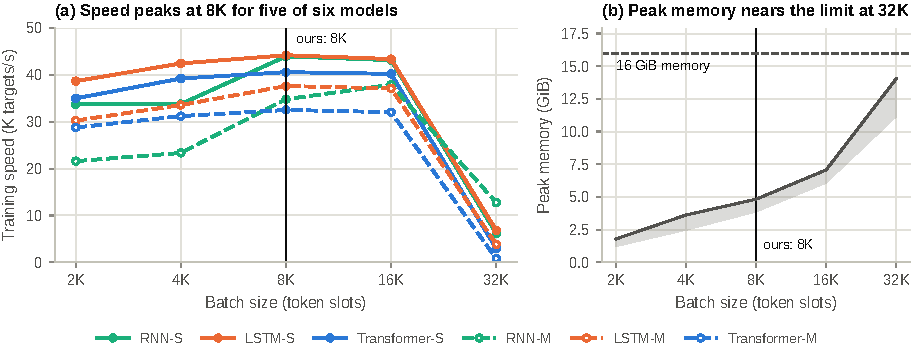
\includegraphics[width=\textwidth]{batch_size.pdf}
\caption{Test-run speed and memory by batch size. (a)~Training speed of the six candidate models; solid lines are the main size (S), dashed lines the size check (M). (b)~Peak memory over the six models: the band is their range and the line the largest. We use 8K positions per batch: the largest size that still raised speed for five of six models, below every step-300 estimate of the gradient noise scale.}
\label{fig:batch}
\end{figure*}

\paragraph{Test run.}
Before the real runs, a 28-minute test run trained each candidate model for 300 steps (about 0.2 epochs) at 8,192 positions per batch and a peak learning rate of $10^{-3}$, on products with keys below 0.45 and with its own vocabulary ($|V| = 16{,}270$); it validated on keys 0.45 to 0.5. It timed 10 steps at five batch sizes, logged unclipped gradient norms, and estimated the gradient noise scale $B_{\text{simple}}$ after 50, 150 and 300 steps from 8 micro-batches \citep[App.~A.1]{mccandlish2018empirical}. It set three values (Table~\ref{tab:pilot}, Figure~\ref{fig:batch}).
\emph{Batch size:} speed rises up to 8K positions for every model and is flat or lower at 16K for five of six (RNN-M gains 9\%); at 32K, memory reaches 11.1 to 14.1~GiB of 16~GiB and speed collapses. At step 300, $B_{\text{simple}}$ is at least 8,060 targets for every model, while an 8K batch holds about 7,150 targets and a 16K batch about 14,000, so 8K is the largest size below every step-300 estimate. The estimates are noisy: at step 150, RNN-M's was 5,977, and LSTM-S's was undefined because its estimate of the squared gradient norm $|G|^2$ came out negative. The throughput plateau therefore decides, and the noise scale only supports it.
\emph{Clipping:} 1.0 lies within half to ten times every model's mean gradient norm over the second half of the run, 0.67 to 1.21 \citep{pascanu2013difficulty}. The vanilla RNNs clip most often (23\% and 41\% of late steps) because their typical norm is near 1.0 (late means 0.96 and 1.21). Adam scales each step by a running average of gradient size, so we expect clipping to change little beyond trimming the largest steps; this is not tested.
\emph{Validation cost:} one validation pass took 8 to 10\,s. Evaluation time, including the training sample scored at each check, is logged separately and left out of training time.





\paragraph{$n$-gram models.}
Kneser-Ney uses the closed-form discounts of \citet[eq.~26]{chen1998empirical} for counts of 1, 2, and 3 or more, with continuation counts for the lower orders; $n$-grams that start with \tok{bos} keep their raw counts, as in \citet[3.2]{heafield2013scalable}, because no word can come before \tok{bos}; a discount outside its valid range falls back to 0.5, 1 or 1.5, as in KenLM. Add-$k$ interpolates add-$k$ estimates of every order up to $n$. Its $k$ is searched over powers of ten from $10^{-4}$ to 1, and the grid is extended tenfold while the best value is at an edge; its weights $\lambda$ are fit by EM on validation data, so its validation $J$ is slightly optimistic, but its test $J$ is not. We did not use KenLM, which rejects \tok{unk} in its input. Tests check that every distribution sums to 1 and that our Kneser-Ney matches a slow reference implementation for orders 1 to 4.

\paragraph{Recipe and sources.}
Table~\ref{tab:recipe} lists every setting with its evidence. The test run checked three of them on our data (batch size, clipping and validation cost); the others follow the cited sources, most of which study larger Transformer models with subword tokens.

\begin{table*}[t]
\centering
\small
\begin{tabularx}{\textwidth}{@{}l>{\raggedright\arraybackslash}p{0.33\textwidth}>{\raggedright\arraybackslash}X@{}}
\toprule
Setting & Value & Evidence \\
\midrule
Tuning & Peak learning rate per model, starting from $\{3\times10^{-4}, 10^{-3}, 3\times10^{-3}\}$ and stepping half a decade further while the best is the largest or smallest tried (range $10^{-5}$ to 0.1); every try a complete planned run; best try kept & If only one hyperparameter can be tuned, tune the learning rate \citep{goodfellow2016deep}; log-spaced values, and explore beyond the border when the best value lies on it \citep[3.1.1, 3.3.1]{bengio2012practical}; which model looks best depends on the tuning budget, so every model gets the same search rule and the tries are reported \citep{dodge2019show} \\\addlinespace[3pt]
Optimizer & AdamW, $\beta_1 = 0.9$, $\beta_2 = 0.999$, $\epsilon = 10^{-8}$; weight decay 0.1 on weight matrices, none on biases, LayerNorm or $E$ & Adam's suggested defaults \citep{kingma2015adam}; SGD converges much more slowly on attention models \citep{zhang2020adaptive}; no newer optimizer consistently beats Adam \citep{schmidt2021descending}; decoupled decay \citep{loshchilov2019decoupled}; 0.1 as in GPT-3 \citep{brown2020language} \\\addlinespace[3pt]
Batch & 8,192 positions including padding (about 7,000 targets in the real runs) for every model & Speed peaks at 8K for five of six models (Figure~\ref{fig:batch}); below every step-300 noise-scale estimate \citep{mccandlish2018empirical}; one size for all, because the best learning rate changes with the batch size \citep{shallue2019measuring} \\\addlinespace[3pt]
Schedule & Linear warm-up over 4\% of steps, then one cosine curve to 10\% of the peak at the planned last step & Adam's early steps have high variance \citep{liu2020variance}; 4,000 of 100,000 steps in \citet{vaswani2017attention}; cosine form of \citet{loshchilov2017sgdr}; overshooting the run by more than 25\% hurts, and decaying 10 times is slightly better than decaying to 0 \citep{hoffmann2022training} \\\addlinespace[3pt]
Clipping & Global gradient norm 1.0 & Half to ten times the mean norm can still converge \citep{pascanu2013difficulty}; test-run means 0.67 to 1.21 (Table~\ref{tab:pilot}); GPT-3 also clips at 1.0 \citep{brown2020language} \\\addlinespace[3pt]
Stopping & Validation $J$ 4 times per epoch; stop after 3 checks without a new best; keep the best checkpoint & Patience-based early stopping \citep[Alg.~7.1]{goodfellow2016deep}; validation curves almost always have more than one local minimum \citep{prechelt1998early} \\\addlinespace[3pt]
Run length & 6 epochs (about 66M targets) per run, for every model and try & The longest run that lets all three models finish their tries overnight on our machine; the course demos also train for a fixed number of epochs (6 in Lecture3\_Demo); rule~2 below tests the budget \\\addlinespace[3pt]
Dropout & 0 in every model & 0.35 parameters (word tables included) per training target, against 26 and 16 for AWD-LSTM on Penn Treebank and WikiText-2 \citep{merity2018regularizing,merity2017pointer}; overfitting is measured, rule~1 below \\\addlinespace[3pt]
Model details & Whole reviews, no truncated backpropagation; one recurrent layer; LSTM forget-gate bias 1; Transformer: ReLU feed-forward, final LayerNorm, token vectors scaled by $\sqrt{d_{\text{model}}}$; $E$ uniform in $\pm 0.1$ with a zero \tok{pad} row & Forget-gate bias \citep{jozefowicz2015empirical}; Transformer as in \citet{vaswani2017attention} with pre-LN \citep{xiong2020layer}, as in GPT-2 \citep{radford2019language}; projection before the output layer \citep{sak2014long,jozefowicz2016exploring} \\\addlinespace[3pt]
Seed & 4213 for initialisation, data order and samples & \\
\bottomrule
\end{tabularx}
\caption{The shared training recipe of the three neural models, with its evidence.}
\label{tab:recipe}
\end{table*}

\paragraph{Rules fixed before any result.}
\label{app:rules}
Three rules were written down before the first run, so the results cannot steer them.
\begin{enumerate}[leftmargin=*,itemsep=1pt,topsep=2pt]
\item \emph{Overfitting.} A model overfits if its validation $J$ stops improving while its training-sample $J$ keeps falling, before the last quarter of its planned run. If any model does, all three get a run with dropout 0.1 on the input embeddings and before the output layer, at their chosen learning rates; if that lowers any model's validation $J$, all three get one more run at 0.3. Main results stay at dropout 0, and the dropout runs are reported next to them.
\item \emph{Training budget.} If a model's validation $J$ still falls in its last epoch by more than the gap to its neighbour in the ranking, all three models get one longer run (10 epochs) at their chosen rates, and both budgets are reported. \todo{If we agreed to run 10 epochs for every model regardless, say so here, and that it was decided after seeing the first try's curve.}
\item \emph{Short tries.} The validation checks show which rate one-epoch tries would have chosen, and whether it matches the full-run winner. Short tries can mislead either way: short horizons favour small step sizes \citep{wu2018understanding}, while the best learning rate falls as training gets longer \citep{bjorck2025scaling}.
\end{enumerate}

\paragraph{Change after the first results.}
The tuning rule fixed before the runs allowed one step past an edge. The LSTM's best rate was then the largest it tried (0.01, after 0.0003, 0.001 and 0.003), so before the Transformer's and RNN's tries finished, we extended the rule for every model: keep stepping half a decade outward while the best rate stays at the edge, as \citet[3.3.1]{bengio2012practical} recommends. The change affects only which rates are tried, and every model's tries are reported. \todo{Fill in what the extended search found.}

\paragraph{Limitations of the recipe.}
The shared settings may suit one model better than another, since only the learning rate is tuned per model. A few tries find a good learning rate, not always the best, and the winner can depend on the tuning budget \citep{dodge2019show}, so we report the tries. Early stopping can end a run before its learning rate has fully decayed, so we report where each run stopped. AdamW may slightly hold back the RNN and LSTM: plain SGD has been reported to work better for LSTM language models \citep{merity2018regularizing}, though that paper does not test Adam itself. The shared 100-number output limits the rank of every model's score matrix \citep{yang2018breaking}, equally for all three, which may shrink the gaps between them; tying $E$ to the output layer would improve perplexity \citep{press2017using} but would freeze the output layer with $E$ in Part~II.

%=====================================================================
\FloatBarrier
\section{Reproducibility, Data and AI Use}
\label{app:repro}

\paragraph{Code and reproducibility.}
\todo{Repository link; the README lists the data download, every command, the configurations and the seed. Python 3.12, PyTorch 2.14.1, dependencies pinned in \texttt{uv.lock}; every run records its git commit, configuration, device and machine; the test suite (number of tests) passes.}

\paragraph{Data.}
Amazon Reviews 2023 states no licence, so the repository holds only the download script, never the data, and we cite the dataset \citep{hou2024bridging}; files that quote reviews stay on the author's machine. \todo{Licences of fastText lid.176 and GloVe 2024 (Part~II).}

\paragraph{AI use.}
\todo{Author's own statement. Draft from the project notes, to rewrite: Claude (Anthropic) wrote the code, its tests and the measurement scripts I ran, and drafted text that I rewrote. I made every decision, ran every experiment and hand-checked the samples; Claude's counts agreed with mine on 7 of 8 samples.}

\end{document}
